\documentclass[aspectratio=169, 12pt]{beamer}
\usepackage{bbm}
\usepackage[utf8]{inputenc}
\usepackage[T2A]{fontenc}
\usepackage[english]{babel}
\usepackage{amscd,amssymb}
\usepackage{amsfonts,amsmath,array}
\usepackage{sidecap}
\usepackage[T2A]{fontenc}
\usepackage[utf8]{inputenc}
\usepackage{graphicx}				% Вставка картинок правильная
\graphicspath{{pictures/}, {images/}, {}}
\DeclareGraphicsExtensions{.pdf,.png,.jpg}
\usepackage{pdfpages}
\usepackage{multicol}

% Для алгоритмов
\usepackage{amsmath}
\usepackage{amsthm}
\usepackage{amssymb}
\usepackage{mathtools}
\usepackage{algorithm}
\usepackage{algpseudocode}
% Цвета 
\usepackage{color}
\usepackage{colortbl}

% Создаем новую команду для assumptions
%----------------------------------------------------------------------------------------------------------

\newtheorem{assumption}{Assumption}
%beamer  theme's used to be here :)
%\usetheme{mipt_beamer}
\usetheme{boxes}

%----------------------------------------------------------------------------------------------------------
\title[\hbox to 56mm{Feature}]{Methods with preconditioning and weight decaying}
\author[M.\,K.~Kreinin]{Matvei Kreinin}
\institute{Moscow Institute of Physics and Technology}
\date{\footnotesize
A. Beznosikov
\par\bigskip\small 2023}

\begin{document}
\maketitle

\begin{frame}{Problem statement}

    Minimize function:
    \begin{equation}
    \label{eq:general}
        \min_{w \in \mathbb{R}^d} f(w)
    \end{equation} 
    
    The classic approach to the solution of minimize function:
    \begin{equation*}
        w_t = w_{t-1} - \eta \nabla f(w_t).
    \end{equation*}

    Preconditioned algorithms:
    \begin{equation*}
        w_{t+1} = w_t - \eta D_t^{-1}g_t
    \end{equation*}
    where $g_t$ is an unbiased stochastic gradient, $D_t$ is a matrix of preconditioning.
    
    
\end{frame}

\begin{frame}{Different ways of matrix with preconditioning}
    AdaGrad:
    \begin{equation*}
        D_t = diag \left\{\sqrt{\sum\limits_{i=0}^t g_i \odot g_i} \right\}
    \end{equation*}
    RMSProp and Adam:
    \begin{equation*}
        D_t^2 = \beta D_{t-1}^2 + (1-\beta) diag \{g_t \odot g_t \}
    \end{equation*}
    OASIS:
    \begin{equation*}
        D_t = diag \{z \odot \nabla^2 f(w_t) z\}
    \end{equation*}
    where $z$ is a random vector from Randamaher distribution.
\end{frame}


\begin{frame}[shrink]{New minimizing function}
\begin{equation*}
        \min_{w \in \mathbb{R}^d} F(w) := f(w) + r(w)
\end{equation*}
where $r(w)$ is a the regularization function.

\begin{algorithm}[H]
    \caption{Different ways of using preconditioning for regularized problem}
    \label{alg:precond}
    
    \begin{algorithmic}
            \Require{$\eta$ $-$ learning rate, $f$ $-$ objective function}
            
            \While {$w$ not converged}
            \State $t = t+1$
            \State $g_t \gets$ stochastic gradient of $f$
            \State $\textcolor{blue}{g_t \gets g_t + \nabla r(w_t)}$ \hfill \textcolor{blue}{standart regularization}
            \State $D_t \gets$ preconditioning matrix, based on $g_t$

            \State \textcolor{blue}{$w_t \gets w_{t-1} - \eta \cdot D_t^{-1}g_t $} \hfill \textcolor{blue}{standart regularization}, 
            \State \textcolor{orange}{$w_t \gets w_{t-1} - \eta \cdot D_t^{-1} \left(g_t +\nabla r(w_t) \right)$} \hfill \textcolor{orange}{scaled weight decay}, 
            \State \textcolor{red}{$w_t \gets w_{t-1} - \eta \cdot D_t^{-1} g_t  - \eta \cdot \nabla r(w_t)$} \hfill \textcolor{red}{weight decay}, 
            \EndWhile
    \end{algorithmic}
\end{algorithm}

\end{frame}

\begin{frame}{Again new target function}
Put $D_t^{-1}$ out of brackets and get new target function:
\begin{equation*}
    w_{t+1} = w_t - \eta D_t^{-1}(\nabla f(w_t) + D_t \nabla r(w_t))
\end{equation*}
A new regularization function $\nabla \tilde{r}(w) = D_t \nabla r(w)$.


New target function:
\begin{equation*}
    \min_{w \in \mathbb{R}^d} \tilde{F}(w) := f(w) + \tilde{r}(w)
\end{equation*}
,where $\tilde{F}(w)$ changes every time step.
\end{frame}

\begin{frame}{Assumptions}

\begin{assumption}[Regularizer structure]
    \label{ass:regstruct}
    Regularizer $r$ is separable, i.e. it can be viewed in the form:
    $$r(w) = \sum_{i=1}^d r_i(w_i).$$
\end{assumption}

\begin{assumption}[Preconditioner structure]
    \label{ass:precondstruct}
    Preconditioner $D_t$ can be viewed in the following form:
    \begin{equation*}
         D_t = \textrm{diag} \left\{ d_t^1 \ldots, d
_t^d \right\}.\end{equation*}
\end{assumption}
\end{frame}

\begin{frame}{Assumptions}
    \begin{assumption}[$L$-smoothness]
\label{ass:smoothness}
\begin{itemize}
    \item 	The gradients of $f$ are $L_f$-Lipschitz continuous $\forall w \in \mathbb{R}^d$, i.e. there exists a constant $L_f > 0$ such that $\forall x, y \in \mathbb{R}^d$,
    	\begin{equation*}
    		f(x) \leq f(y) + \langle \nabla f(y), x-y \rangle + \frac{L_f}{2} \|x - y\|^2.
    	\end{equation*}
    \item    The gradient of $r$ is $L_r$-Lipschitz continuous $\forall w \in \mathbb{R}^d$, i.e. there exists a constant $L_r > 0$ such that $\forall x, y \in \mathbb{R}^d$,
	\begin{equation*}
		r(x) \leq r(y) + \langle \nabla r(y), x-y \rangle + \frac{L_r}{2} ||x - y||^2.
	\end{equation*}
\end{itemize}
\end{assumption}
\end{frame}

\begin{frame}[shrink]{Assumptions}
\begin{assumption}[PL--condition]
\label{ass:plcondition}
	There exists $\mu > 0$, such that $\forall w \in \mathbb{R}^d$
    \begin{equation*}
        ||\nabla f(w) || \geq 2 \mu (f(w) - f^*).
    \end{equation*}
\end{assumption}

\begin{assumption}[Preconditioner]
Restrictions on preconditioner $D_t$
\label{ass:preconditioned}
\begin{equation*}
\alpha I \preccurlyeq D_t \preccurlyeq \Gamma I \Leftrightarrow \frac{I}{\alpha} \preccurlyeq D_t^{-1} \preccurlyeq \frac{I}{\Gamma}.
\end{equation*}
\end{assumption}

\begin{assumption}[Expectations]
Restrictions on $D_t$ and $g_t$ are unbiased, i.e.
\ref{ass:expectations}
\begin{equation*}
\mathbb{E} \left[ D_t \right] = D_t \text{ and }\mathbb{E}\left[ g_t \right] = \nabla f (w_t), \mathbb{E}\left[ ||g_t - \nabla f||^2 \right] \leq \sigma^2.
\end{equation*}
\end{assumption}
    
\end{frame}

\begin{frame}{Lemmas}
    \begin{lemma}[Existence of $\widetilde{r}$]
    Suppose the Assumptions \ref{ass:regstruct}, \ref{ass:precondstruct} hold, the function $\widetilde{r}$ exists and has following form:
    $$\widetilde{r}(w) = \sum_{i=1}^d d_t^i r_i(w_i)$$
\end{lemma}

\begin{lemma}[L-smoothness of $\widetilde{r}$]
Suppose the Assumptions \ref{ass:regstruct}, \ref{ass:precondstruct}, \ref{ass:smoothness} hold,
The gradient of $\widetilde{r}$ is $L_{\tilde{r}}$-continuous, i.e.  there exists a constant $L_{\tilde{r}} > 0$ such that $\forall x, y \in \mathbb{R}^d$,
    	\begin{equation*}
    		\widetilde{r}(x) \leq \widetilde{r}(y) + \langle \nabla \widetilde{r}(y), x-y \rangle + \frac{L_{\tilde{r}}}{2} ||x - y||^2,
    	\end{equation*}
     where $L_{\tilde{r}} = ||D_t|| L_r$
\end{lemma}
\end{frame}
\if 0
\begin{frame}{Lemmas}
    \begin{lemma}\label{lemma:lowerbondF}{Lower bound}
Suppose the Assumptions \ref{ass:regstruct}, \ref{ass:precondstruct} and \ref{ass:smoothness} holds, then difference between a solution $w^*$ of a problem \eqref{F_big} and a solution $\widetilde{w}^*$ of a problem \eqref{F_tilde} can be bounded below.
    \begin{equation*}
        \|\widetilde{w}^* - w^* \| L_F \geq \| \nabla r (\widetilde{w}^*) (I - D_t)\|
    \end{equation*}
\end{lemma}
\end{frame}
\fi 

\begin{frame}{Theorems}
\begin{theorem}[1]
\label{theor:1}
    Suppose the Assumptions \ref{ass:smoothness}, \ref{ass:preconditioned} hold, let $\varepsilon > 0$ and let the step-size satisfy, where $L_f, L_{\tilde{r}}$ - lipschitz constants of functions $f$ and $\tilde{r}$, $\alpha I \preccurlyeq D_t \preccurlyeq \Gamma$
    \begin{equation*}
        \eta < \frac{2 \alpha}{L_f + \Gamma L_{\tilde{r}} \alpha}.
    \end{equation*}
    Then, the number of iterations performed by algorithms with preconditioning and weight decaying, starting from an initial point $w_0 \in \mathbb{R}^d$ with $\Delta_0 = \tilde{F}(w_0) - \tilde{F}^*$, required to obtain and $\varepsilon$-approximate solution of the convex problem \eqref{eq:general} can be bounded by
    \begin{equation*}
          T = \mathcal{O}\left( \frac{2\Delta_0 \Gamma \alpha } {\left(2\alpha - \left( L_f + \Gamma L_{\tilde{r}} \alpha \right)\eta \right) \eta \varepsilon} \right).
    \end{equation*}
\end{theorem}
\end{frame}

\begin{frame}{Theorems}
    \begin{theorem}
\label{theor:2}
    Suppose the Assumptions \ref{ass:smoothness}, \ref{ass:plcondition}, \ref{ass:preconditioned} hold, let $\varepsilon > 0$ and let the step-size satisfy, where $\alpha I \preccurlyeq D_t \preccurlyeq \Gamma$, $L_{\tilde{F}} = L_{f} + \Gamma L_{r}$, and $L_{F}, L_{r}$ - lipschitz constant of functions $f$ and $r$, 
    \begin{equation*}
        \eta \leq \frac{2 \alpha}{L_{\widetilde{F}}}.
    \end{equation*}
    Let $\tilde{F}^*$ be a solution of the optimization function. Then, the number of iterations performed by algorithms with preconditioning and weight decaying, starting from an initial point $w_0 \in \mathbb{R}^d$ with $\Delta_0 = \tilde{F}(w_0) - \tilde{F}^*$, required to obtain and $\varepsilon$-approximate solution of the convex problem \eqref{eq:general} can be bounded by
    \begin{equation*}
        T =  \mathcal{O}\left( \frac{\ln \frac{\Delta_0}{\epsilon}}{2 \mu \eta^2 \left(\frac{1}{\eta} - \frac{L_{\tilde{F}}}{2 \alpha} \right)} \right).
    \end{equation*}
\end{theorem}
\end{frame}

\begin{frame}[shrink]{Theorems}
    \begin{theorem}[3]
    Suppose the Assumptions \ref{ass:smoothness}, \ref{ass:plcondition}, \ref{ass:preconditioned}, \ref{ass:expectations} hold, let $\varepsilon > 0$ and let the step-size satisfy
    \begin{equation*}
        \eta \approx \sqrt{\frac{\left( \tilde{F}(w_0) - \tilde{F}(w_*) \right)\alpha}{L \sigma^2}}.
    \end{equation*}
    Let $\tilde{F}^*$ be a solution of the optimization function. Then, the number of iterations performed by algorithms with preconditioning and weight decaying, starting from an initial point $w_0 \in \mathbb{R}^d$ with $\Delta_0 = \tilde{F}(w_0) - \tilde{F}^*$, required to obtain and $\varepsilon$-approximate solution of the convex problem \eqref{eq:general} can be bounded by, where $L_{\tilde{r}}, L_{f}$ - lipschitz constant of functions $\tilde{r}$ and $f$, and $L_{\tilde{F}} = L_{f} + \Gamma L_{r}$
    
    \begin{equation*}
        T =  \mathcal{O}\left( \frac{\Gamma \Delta_0}{\left(\frac{1}{\eta} - \frac{ \Gamma L_{\tilde{r}}}{2} - \frac{\Gamma L_{\tilde{F} }L_{f}\eta^2}{2\alpha^2} \right) \varepsilon} \right).
\end{equation*}
    \label{theor:3}
\end{theorem}
\end{frame}

\begin{frame}{AdamW}
    \begin{algorithm}[H]
            \caption{Adam}\label{alg:genAdam}    
            \begin{algorithmic}
            \small{
            \Require{$\eta, \beta_1, \beta_2, \epsilon, f, r$}
            %\State $m_0 = 0$ -- 1-st moment vector
            %\State$v_0 = 0$ -- 2-nd moment vector
            \While {$\theta$ not converged}
            \State $t = t+1$
            \State $g_t = \nabla f(w_{t-1}) + $ \textcolor{blue}{$\nabla r(w_{t-1})$}\hfill \textcolor{blue}{AdamL2}
            \State $m_t = \beta_1 \cdot m_{t-1} + (1 - \beta_1) \cdot g_t$
            \State $v_t = \beta_2 \cdot v_{t-1} + (1 - \beta_2) \cdot g_t^2$
            \State $\hat{m_t} = \frac{m_t}{1-\beta_1^t} +$ \textcolor{orange}{$\nabla r(w_{t-1})$} \hfill \textcolor{orange}{AdamWH}
            \State $\hat{v_t} = \frac{v_t}{1-\beta_2^t}$ 
            \State $w_t = w_{t-1} - \eta \cdot \frac{\hat{m_t}}{\sqrt{v_t} + \epsilon} - $ \textcolor{red}{$\eta \nabla r(w_{t-1})$ } \hfill \textcolor{red}{AdamW}
            \EndWhile
            }
\end{algorithmic}
\end{algorithm}
\end{frame}

\begin{frame}{OASIS}
    \begin{algorithm}[H]
\caption{OASIS}\label{alg:OASIS}
\begin{algorithmic}
    \Require{$w_0, \eta_0, D_0, \theta_0 = + \infty$}    
    \State $w_1 = w_0 - \eta \hat{D_0}^{-1} \nabla f(w_0)$

    \For{$k = 1, 2, ...$}
    \State $g_k = \nabla f(w_k) +$ \textcolor{blue}{$\nabla r(w_{t-1})$}\hfill \textcolor{blue}{OASISL2} 
    \State $D_k = \beta D_{k-1} + (1-\beta_2) \cdot diag\left( z_k \odot \nabla^2 \left(f(w_k) + \textcolor{orange}{r(w_k)} \right) z_k \right)$ \hfill \textcolor{orange}{OASISWH}
    \State $(\hat{D_k})_{ii} = max \{|D_k|_{i, i} ; \alpha \}$, $\forall i = \overline{1, d}$
    \State $\eta_k = min \{ \sqrt{1 + \theta_{k-1}} \cdot \eta_{k-1}; \frac{||w_k - w_{k-1}||_{\hat{D_k}}}{2 ||\nabla f(w_k) - \nabla f(w_{k-1}) ||_{\hat{D_k}}^* } \}$
    \State $w_{k+1} = w_k - \eta_k g_k D_k^{-1}- $ \textcolor{red}{$\eta \nabla r(w_{t-1})$ } \hfill \textcolor{red}{OASISW} 
    \State $\theta_k = \frac{\eta_k}{\eta_{k-1}}$
    \EndFor
    
\end{algorithmic}
\end{algorithm}
\end{frame}

\begin{frame}{Experiments}
   \begin{figure}[H]
\begin{minipage}[h]{0.49\linewidth}
\centering
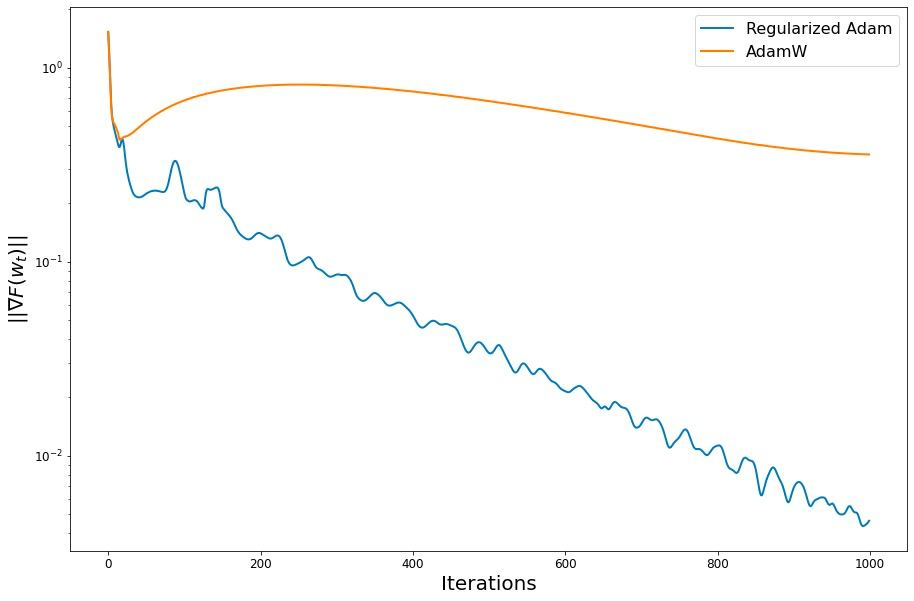
\includegraphics[width=\linewidth]{adams_errors.jpeg}

\caption{Adam and AdamW with basic criterion}
\label{fig:adams_errors}
\end{minipage}
\hfill
\begin{minipage}[h]{0.49\linewidth}
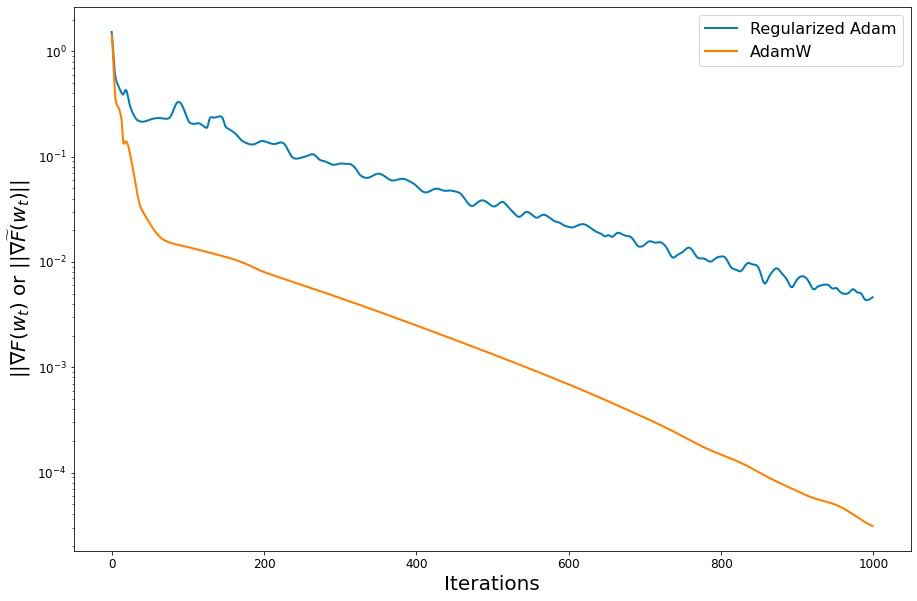
\includegraphics[width=\linewidth]{adams_special_errors.jpeg}

\caption{Adam and AdamW with modified criterion}
\label{fig:adams_special_errors}
\end{minipage}
\end{figure}
\end{frame}

\begin{frame}[shrink]{Experiment}
\begin{columns}[T]
\column{0.7\textwidth}

\begin{center}
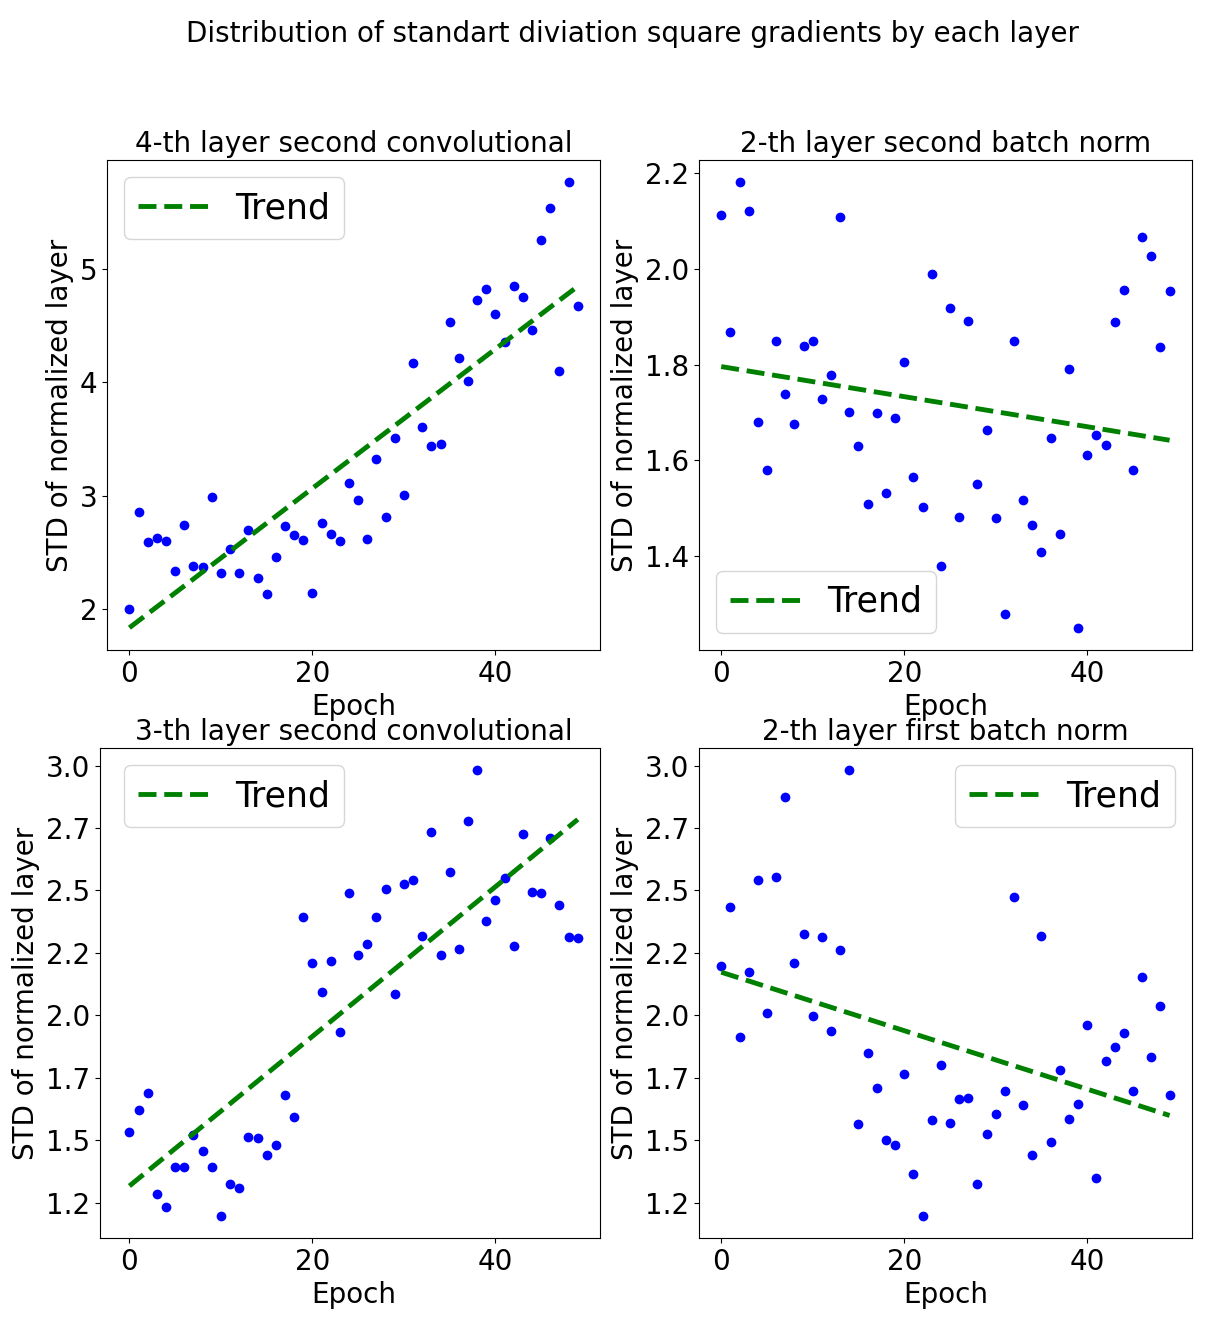
\includegraphics[scale=0.18]{new_layers.png}
    
    Distribution of standard deviation of elements of matrix $D_t$ over epochs. 
\end{center}
\column{0.3\textwidth}
\begin{center}
  Deviation of the normalized weights in the convolutional layers has rising trend. Hence, difference
between solutions of different problems is bounded below and methods converge to a different optimums.
\end{center}
\end{columns}
\end{frame}


\begin{frame}{Publications:}
    \begin{itemize}
        \item Kingma, Diederik P., and Jimmy Ba. "Adam: A method for stochastic optimization." arXiv preprint arXiv:1412.6980 (2014).
        \item Jahani, Majid, et al. "Doubly adaptive scaled algorithm for machine learning using second-order information." arXiv preprint arXiv:2109.05198 (2021).
        \item Sadiev, Abdurakhmon, et al. "Stochastic gradient methods with preconditioned updates." arXiv preprint arXiv:2206.00285 (2022).
        \item Beznosikov, Aleksandr, et al. "On scaled methods for saddle point problems." arXiv preprint arXiv:2206.08303 (2022).
        \item Loshchilov, Ilya, and Frank Hutter. "Decoupled weight decay regularization." arXiv preprint arXiv:1711.05101 (2017).
        \item Xie, Zeke, Issei Sato, and Masashi Sugiyama. "Stable weight decay regularization." (2020).
    \end{itemize}
\end{frame}

\begin{frame}{Conclusion:}
    \begin{itemize}
        \item Proposed novel approach how to apply weight decaying in algorithm.
        \item Theorethical analyse of convergency of methods with preconditioning and weight decaying. 
        \item Create new optimization algorithm AdamWH.
        \item 3 theorems and 2 lemmas for estimating the convergence of methods with preconditioning and weight decaying are proved 
        \item The further direction of analyzing the distribution of preconditioning elements in neural networks, another direction is to make a coordinate adam in neural networks.
    \end{itemize}
\end{frame}


\end{document}